% Options for packages loaded elsewhere
\PassOptionsToPackage{unicode}{hyperref}
\PassOptionsToPackage{hyphens}{url}
%
\documentclass[
]{article}
\usepackage{amsmath,amssymb}
\usepackage{lmodern}
\usepackage{ifxetex,ifluatex}
\ifnum 0\ifxetex 1\fi\ifluatex 1\fi=0 % if pdftex
  \usepackage[T1]{fontenc}
  \usepackage[utf8]{inputenc}
  \usepackage{textcomp} % provide euro and other symbols
\else % if luatex or xetex
  \usepackage{unicode-math}
  \defaultfontfeatures{Scale=MatchLowercase}
  \defaultfontfeatures[\rmfamily]{Ligatures=TeX,Scale=1}
\fi
% Use upquote if available, for straight quotes in verbatim environments
\IfFileExists{upquote.sty}{\usepackage{upquote}}{}
\IfFileExists{microtype.sty}{% use microtype if available
  \usepackage[]{microtype}
  \UseMicrotypeSet[protrusion]{basicmath} % disable protrusion for tt fonts
}{}
\makeatletter
\@ifundefined{KOMAClassName}{% if non-KOMA class
  \IfFileExists{parskip.sty}{%
    \usepackage{parskip}
  }{% else
    \setlength{\parindent}{0pt}
    \setlength{\parskip}{6pt plus 2pt minus 1pt}}
}{% if KOMA class
  \KOMAoptions{parskip=half}}
\makeatother
\usepackage{xcolor}
\IfFileExists{xurl.sty}{\usepackage{xurl}}{} % add URL line breaks if available
\IfFileExists{bookmark.sty}{\usepackage{bookmark}}{\usepackage{hyperref}}
\hypersetup{
  pdftitle={DAEDALUS: economic variables},
  hidelinks,
  pdfcreator={LaTeX via pandoc}}
\urlstyle{same} % disable monospaced font for URLs
\usepackage[margin=1in]{geometry}
\usepackage{longtable,booktabs,array}
\usepackage{calc} % for calculating minipage widths
% Correct order of tables after \paragraph or \subparagraph
\usepackage{etoolbox}
\makeatletter
\patchcmd\longtable{\par}{\if@noskipsec\mbox{}\fi\par}{}{}
\makeatother
% Allow footnotes in longtable head/foot
\IfFileExists{footnotehyper.sty}{\usepackage{footnotehyper}}{\usepackage{footnote}}
\makesavenoteenv{longtable}
\usepackage{graphicx}
\makeatletter
\def\maxwidth{\ifdim\Gin@nat@width>\linewidth\linewidth\else\Gin@nat@width\fi}
\def\maxheight{\ifdim\Gin@nat@height>\textheight\textheight\else\Gin@nat@height\fi}
\makeatother
% Scale images if necessary, so that they will not overflow the page
% margins by default, and it is still possible to overwrite the defaults
% using explicit options in \includegraphics[width, height, ...]{}
\setkeys{Gin}{width=\maxwidth,height=\maxheight,keepaspectratio}
% Set default figure placement to htbp
\makeatletter
\def\fps@figure{htbp}
\makeatother
\setlength{\emergencystretch}{3em} % prevent overfull lines
\providecommand{\tightlist}{%
  \setlength{\itemsep}{0pt}\setlength{\parskip}{0pt}}
\setcounter{secnumdepth}{5}
\usepackage{eso-pic,graphicx,transparent}
\ifluatex
  \usepackage{selnolig}  % disable illegal ligatures
\fi
\newlength{\cslhangindent}
\setlength{\cslhangindent}{1.5em}
\newlength{\csllabelwidth}
\setlength{\csllabelwidth}{3em}
\newenvironment{CSLReferences}[2] % #1 hanging-ident, #2 entry spacing
 {% don't indent paragraphs
  \setlength{\parindent}{0pt}
  % turn on hanging indent if param 1 is 1
  \ifodd #1 \everypar{\setlength{\hangindent}{\cslhangindent}}\ignorespaces\fi
  % set entry spacing
  \ifnum #2 > 0
  \setlength{\parskip}{#2\baselineskip}
  \fi
 }%
 {}
\usepackage{calc}
\newcommand{\CSLBlock}[1]{#1\hfill\break}
\newcommand{\CSLLeftMargin}[1]{\parbox[t]{\csllabelwidth}{#1}}
\newcommand{\CSLRightInline}[1]{\parbox[t]{\linewidth - \csllabelwidth}{#1}\break}
\newcommand{\CSLIndent}[1]{\hspace{\cslhangindent}#1}

\title{DAEDALUS: economic variables}
\author{}
\date{\vspace{-2.5em}25 May, 2023}

\begin{document}
\maketitle

{
\setcounter{tocdepth}{5}
\tableofcontents
}
\AddToShipoutPictureFG{
  \AtPageCenter{% or \AtTextCenter
    \makebox[0pt]{\rotatebox[origin=c]{45}{%
      \scalebox{7}{\texttransparent{0.3}{PRELIMINARY DRAFT}}%
    }}
  }
}

\hypertarget{introduction}{%
\section{Introduction}\label{introduction}}

The objective of the proposed work is to use scenario modelling to ascertain the vulnerability of a country to a hypothetical pandemic across several dimensions. The dimensions of vulnerability we consider here include economic loss, life loss, and education loss. The variables we consider as potential indicators of vulnerability relate to the reliance of the economy on two economic sectors, and the level of digitization and associated capacity to provide home-based work and education.

We simulate hypothetical pandemics caused by one of seven respiratory pathogens, each with a disease profile informed by a past epidemic. We use the integrated epi-econ model DAEDALUS developed in our group for estimating the benefit of pandemic preparedness (P2) (Haw et al. 2022). The scenarios are informed by real-world demographic, societal and economic data for up to 197 countries. We evaluate outcomes for four mitigation strategies (``unmitigated,'' ``adaptive economic closures,'' ``school closures,'' and ``elimination'').

The impacts we project are losses to life, to education, and to GDP. We assess the impacts of the four variables of interest on the outcomes using value-of-information methods in order to identify which variables most influence outcomes, and in what circumstances.

\hypertarget{methods}{%
\section{Methods}\label{methods}}

\hypertarget{scenarios}{%
\subsection{Scenarios}\label{scenarios}}

The seven pathogen profiles include influenza and coronaviruses, and are based on past epidemics. Influenza virus profiles correspond to pandemics of the years 1918, 1957 and 2009. Coronavirus profiles correspond to SARS-CoV-1 and SARS-CoV-2, with three profiles: one, corresponding to variants that predated the variant-of-concern nomenclature (which we label ``pre-alpha''), and one each for the Delta and Omicron variants.

The four mitigation strategies are ``unmitigated,'' ``adaptive economic closures,'' ``school closures,'' and ``elimination.'' In the unmitigated strategy, no aversive actions are taken. With adaptive economic closures, sectors close according to a pre-specified programme when hospital occupancy approaches its capacity. With school closures, schools remain closed and other economic sectors have reduced operations. With the elimination strategy, stringent economic closures are maintained until case numbers can be contained by a testing programme. All economic configuration profiles are based on GVA profiles observed in 2020, where the monthly GVA of a sector relative to its value one year prior is interpreted as the degree to which it was open.

We consider three stylised ``countries'' and parametrise models using data from constituent countries according to the World Bank income-classification categories:

\begin{itemize}
\tightlist
\item
  LLMIC, using inputs from LICs and LMICs
\item
  MIC, using inputs from LMICs and UMICs
\item
  HIC, using inputs from HICs
\end{itemize}

\hypertarget{outcomes}{%
\subsection{Outcomes}\label{outcomes}}

The outcomes of the model are:

\begin{enumerate}
\def\labelenumi{\arabic{enumi}.}
\tightlist
\item
  Number of deaths (by four age groups)
\item
  GDP loss
\item
  Education loss
\end{enumerate}

Numbers of deaths are translated into years of life lost (YLL). This takes into account the life expectancy of each person who dies. YLLs are valued using the value of a statistical life, which we estimate as being 160 times GDP per capita (Robinson, Hammitt, and O'Keeffe 2019).

GDP loss is estimated as the total GDP - the sum of GVA across all sectors, scaled by how open they are across the year - divided by the value of GDP when all sectors are completely open all the time.

Education loss takes into account the extent to which schools are closed, as well as the effectiveness of provision for remote learning. We estimate this using internet coverage as a proxy (that is, we do not take into account education that can be delivered by TV or radio). Education loss is valued by taking into consideration life-long earning losses, following (Psacharopoulos, Collis, and Patrinos 2021).

We report these outcomes as a percentage of GDP (for the year prior to the pandemic -- here, 2019). All three outcomes (once a valuation is applied) are linear functions of GDP, and therefore results are all comparable across countries. The time horizon in the simulation is one year.

\hypertarget{modelling}{%
\subsection{Modelling}\label{modelling}}

The integrated epi-econ model is used to project economic and epidemic outcomes. The epidemiological model is a population-structured compartmental SEIR model. It takes many inputs, including pathogen natural history parameters (such as R\(_0\), case-fatality rates, etc) and population parameters (such as age structure, contact rates, etc). The economic model takes as input the GVA per sector, which uses the OECD classification of 45 economic sectors. Both models take as input the economic configuration over time: this is the extent to which each sector is open in each month. A sector is open to a maximum amount of 100\%, when its full monthly GVA value is realised. If a sector is open to 50\%, it contributes 50\% of its maximum GVA that month. In the epidemic model, contacts associated with that sector -- between workers, from workers to consumers, and between consumers -- are likewise scaled down.

The economic model is very simple: we do not model interdependencies between sectors, and the only way in which country interdependencies are taken into account is via changes to tourism which manifest in the ``food and accommodation services'' sector (see Section \ref{impact-of-tourism}). We do not model seasonality or allow for sectors to grow (either in GDP or in workforce).

We generate a distribution over outcomes through sampling inputs. This distribution represents a catalogue of synthetic countries whose characteristics are randomly taken from candidate countries. By examining the relationships between inputs and outputs, we can identify the inputs that most drive uncertainty in outputs as encoded by our model or, equivalently, which inputs are the best predictors of the outcome(s), independently of all other variables.

We include uncertainty in as many parameters as possible. We sample from specified distributions, or sample with replacement from a discrete set of candidate options, where the candidate options are the values belonging to countries in the income group.

Parameter distributions are independent of each other (with the exception of loss in tourism, where the size of the sector is related to the fraction of tourism that comes in from abroad (see Section \ref{loss-of-international-tourists})). This means that any relationships we uncover between input and output within an income group will be causal, and we will not discover any factors that are ``indicative'' by association. (Between income groups there are many systematic differences in inputs and learning which of those drives the differences in outcomes is part of the ongoing development of the model.)

\hypertarget{value-of-information}{%
\subsection{Value of information}\label{value-of-information}}

We assess the impacts of four parameters that relate to economic indicators:

\begin{enumerate}
\def\labelenumi{\arabic{enumi}.}
\tightlist
\item
  Agricultural GVA as a proportion of GDP
\item
  Tourism GVA as a proportion of GDP
\item
  Proportional of tourism that comes from abroad
\item
  Internet coverage
\end{enumerate}

We use value-of-information methods to quantify these relationships. Specifically, we estimate the expected value of partial perfect information (EVPPI), which is the expected gain (in terms of reduction of uncertainty in the outcome) of knowing a parameter (or set of parameters) perfectly (Jackson et al. 2021). Equivalently, and in terms of identifying indicators of vulnerability, it tells us which parameters best predict the outcome.

Value of information is a decision-theoretic quantity. We estimate it using the R package \textbf{voi}. Intuitively, EVPPI functions in a similar way to correlation. In the case of a linear relationship between one input and one output, the computation of EVPPI is essentially the same as that of a correlation. EVPPI extends a simple correlation analysis in two ways relevant to the results presented: 1) nonlinear relationships are also captured, and 2) we can assess the EVPPI of a set of parameters. While EVPPI allows us to identify important relationships in this way, it also means that we cannot make statements such as ``a 3\% increase in this input leads to a 1\% increase in this outcome.''

Finally, we can use mutual information (MI, via the R package \textbf{infotheo}) to assess mutual information between inputs and outputs. What MI offers beyond EVPPI is that it takes into account also how \emph{likely} it is that the input parameter occupies a space where it is influential.

\newpage

\hypertarget{results}{%
\section{Results}\label{results}}

\hypertarget{distributions-over-outcomes}{%
\subsection{Distributions over outcomes}\label{distributions-over-outcomes}}

Distributions over costs associated with the first year of an outbreak of SARS-CoV-2 (with parameters corresponding to variants arising before alpha) are shown in Figure \ref{fig:prealpha} for three income levels and four mitigation strategies. Each shape represents the probability density made up of the sampled values for outcomes: the most likely value to take is where the figure is widest. The tip of the tail indicates the highest value sampled, after which point the density is 0.

These distributions show that vulnerability to a pandemic depends on a country's income level together with its mitigation strategy. For example, the elimination strategy appears to have the lowest distribution for overall cost for HICs among all strategies, whereas it appears no lower for MICs and perhaps higher for LLMICs. This will be because of the factors that vary systematically across countries of different income levels. Likewise, the heavier tails in the distributions for YLLs for HICs is likely due to the age distributions in HICs being heavier in older ages. These cross-country differences are one of the focuses of the development of the model.

\begin{figure}
\centering
\includegraphics{p2_files/figure-latex/prealpha-1.pdf}
\caption{\label{fig:prealpha}Model results for pre-alpha variants of SARS-CoV-2.}
\end{figure}

``If a hypothetical low- or lower-middle income country that relies to 3\% on tourism for their national income experienced a pandemic with a similar profile to the Spanish Flu, what would be the number of deaths, the loss in GDP, and the loss of in-person schooling were the country to rely on an elimination strategy? What would the impact be if the country relied to 6\% on tourism?''

At 3\%, life-year loss is expected to be 7.94\% of GDP (95\%PI 0, 71.98). Education loss is expected to be 29.91\% of GDP (95\%PI 1.24, 68.14). GDP loss is expected to be 15.87\% of GDP (95\%PI 2.48, 24.87).

At 6\%, life-year loss is expected to be 6.04\% of GDP (95\%PI 0, 39.78). Education loss is expected to be 31.01\% of GDP (95\%PI 2.45, 72.47). GDP loss is expected to be 18.16\% of GDP (95\%PI 5.2, 27.19).

Here, the uncertainty in model results swamps the difference in expected values across all outcomes.

\newpage

\hypertarget{value-of-information-1}{%
\subsection{Value of information}\label{value-of-information-1}}

The value of information associated with a number of parameters for all costs considered is shown in Figure \ref{fig:voi}. The costs are listed down the y axis. Parameters and parameter groups are along the x axis. Colours indicate the extent to which uncertainty in the input(s) are driving uncertainty in the outcome, with lighter colours representing greater impact.

The first four items on the x axis are the four independent variables: size of the agriculture sector, size of the food and accommodation services sector, fraction of tourism coming from abroad, and internet coverage. While the two parameters driving tourism are impactful on GDP loss, particularly for strategies light on economic closures, they have little impact on total costs. (This relationship is also driven by the distribution of the food and accommodation sector contribution to GVA: the mutual information appears a more balanced metric (Figure \ref{fig:mi}).) Meanwhile, internet coverage has modest impacts, particularly on education loss and for strategies that employ school closures.

The EVPPI (and MI) for tourism is high, particularly for lower-income countries because tourism can make up a large part of GDP, and particularly for strategies light on economic closure because then the only sector suffering a shortfall is the Food and accommodation services sector.

The next two items on the x axis are parameter groups. First, both sectors. Second, both tourism parameters. The grouping of parameters shows their combined impact on outcomes, which can be greater than the sum of their individual impacts.

The next columns do not correspond to the ``independent variables'' of interest but might be expected to influence outcomes: fraction of population who are school age, fraction of population who are in the oldest age group, population size, rate of testing, GDP, \(R_0\) and maximum hospital capacity. \(R_0\) in particular drives a lot of uncertainty in costs, primarily through YLLs.

The final four items on the x axis are groups of variables: both age groups; two social-distancing parameters; hospital capacity, the fraction of the population aged 65 and over, and R\(_0\); and testing parameters, response time, and R\(_0\).

Some distributions in Figure \ref{fig:prealpha} are bimodal. For example, GDP loss under the Economic Closures strategy have peaks in density close to zero and also far from zero, with a low-density region in between. Here, in some samples (low GDP loss), the epidemic was not severe enough to warrant closures. This could be because R\(_0\) was low, because hospital capacity was high, or both. Similarly, under the Elimination strategy, there is an area of high density at higher costs where the strategy does not work: due to R\(_0\) being high, and/or the capacity to test being low, case numbers are not brought low enough and severe economic closures persist throughout, leading to high GDP loss.

These relationships are identified in the value-of-information analyses: the last two columns show value of information for R\(_0\) and hospital capacity combined, and R\(_0\) and testing rate combined. These variables together explain much of the variance in GDP loss for the Economic Closures and Elimination strategies, respectively.

\begin{figure}
\centering
\includegraphics{p2_files/figure-latex/voi-1.pdf}
\caption{\label{fig:voi}Value of information for pre-alpha variants of SARS-CoV-2.}
\end{figure}

\begin{figure}
\centering
\includegraphics{p2_files/figure-latex/mi-1.pdf}
\caption{\label{fig:mi}Because of the very heavily skewed distribution of the food and accommodation services sector as a share of GDP, mutual information (MI) might be better.}
\end{figure}

\newpage

To understand the relationship between a parameter and an outcome, e.g.~whether the relationship is linear and increasing or decreasing, whether it is nonlinear, whether it is driven by extreme values, they must be plotted against each other. Likewise, a relationship between a parameter pair and an outcome can be plotted, e.g.~Figure \ref{fig:tourismgdp}: for middle-income countries in a pre-alpha SARS-CoV-2 pandemic with the ``No Closures'' strategy, GDP loss is greatest when both the food and accommodation services GVA as fraction of GDP and international tourism as a fraction of tourism are high.

\begin{figure}
\centering
\includegraphics{p2_files/figure-latex/tourismgdp-1.pdf}
\caption{\label{fig:tourismgdp}Relationship between tourism parameters and GDP loss for middle-income countries in a pre-alpha SARS-CoV-2 pandemic with the ``No Closures'' strategy.}
\end{figure}

\newpage

\hypertarget{conclusions}{%
\section{Conclusions}\label{conclusions}}

Using simulation modelling, we have projected distributions of epidemic losses -- of life, GDP, and education -- for seven pathogenic profiles, four stylised mitigation strategies, and three levels of country income. We assessed what the impact is of four economic variables in our model: fraction of GDP from the agriculture sector, fraction of GDP from the food and accommodation services sector, fraction of tourism that comes from abroad, and internet coverage.

We found that the tourism-related variables impacted GDP loss for the No Closure strategy, which is because GDP losses will be suffered only in this sector when there is no mandated closure. This means the GDP loss will depend on the extent to which the economy is depending on this sector. We found that Education losses depend to some extent on internet coverage, because our model assumes that internet access can be used to mitigate losses by enabling remote learning. We found little effect of the size of the agricultural sector.

In parallel, we present a selection of other model parameters, including those related to demography (e.g.~the fraction of the population who are of school age), to the economy (e.g.~GDP), to the health system (e.g.~hospital capacity), to the pandemic response (e.g.~the rate of testing), and to the pathogen (e.g.~the basic reproductive number, R\(_0\)). We found that these variables -- in combinations up to four -- account for much of the variability in outcomes.

\hypertarget{the-modelling-framework}{%
\subsection{The modelling framework}\label{the-modelling-framework}}

Ours is a mechanistic simulation model. The model encodes complex relationships between demographic, epidemic and economic variables. With simulation, it allows us to explore outcomes as consequences of inputs using information- and decision-theoretic methods. Modelling allows \emph{in silico} experimentation, which is crucial for questions pertaining to rare events with small and confounded datasets, as cross-sectional country data are. The model allows us to ask questions about cause and effect that cannot be asked in reality and rarely can be inferred from observational data.

The challenge we face with modelling, then, is to be confident that our model mimics reality, or at least captures the most salient aspects of it.

\hypertarget{the-economic-model}{%
\subsection{The economic model}\label{the-economic-model}}

We have used a simple economic model that allows us to estimate GDP loss in a year assuming that sector closures follow mandates. The mandates we use are schematic and representative of GVA profiles seen in different countries in 2020.

The economic model is static, and does not take into account any dynamics such as feedback, changes to demand, supply and supply chains, changes in international trade, or any macroeconomic factors. As such, to model longer-term economic impacts (apart from the impact of lost education) is beyond the scope of this model.

For example, Figure \ref{fig:gdpdata2} shows the relationship between GDP loss in the first year (2020) and GDP loss in the second year (2021) following the outbreak of COVID-19. There is heterogeneity in losses in the first year, but also in whether or not the economy recovers in the second year, and to what extent. The recovery is arguably a more important phenomenon to capture than initial losses, and it is not something that can be captured by our economic model. However, a model of recovery / future losses would include initial loss as an input, which our model could provide.

\begin{figure}
\centering
\includegraphics{p2_files/figure-latex/gdpdata2-1.pdf}
\caption{\label{fig:gdpdata2}GDP loss and recovery. On the x axis is the GDP of 2020 relative to its 2019 projected value (IMF). On the y axis is 2021 GDP relative to its 2019 projected value relative to the same value for 2020 (ratio of ratios). x values below 100 represent a loss in the year 2020. y values above 0 represent recovery (i.e.~growth exceeded what was expected in 2019); y values equal to zero represent a fixed level of loss; y values less than zero represent increasing loss.}
\end{figure}

\newpage

\hypertarget{references}{%
\section{References}\label{references}}

\hypertarget{refs}{}
\begin{CSLReferences}{1}{0}
\leavevmode\hypertarget{ref-Fraser2009}{}%
Fraser, Christophe, Christl A Donnelly, Simon Cauchemez, William P Hanage, Maria D Van Kerkhove, T Déirdre Hollingsworth, Jamie Griffin, et al. 2009. {``{Pandemic potential of a strain of Influenza A (H1N1): Early findings}.''} \emph{Science} 324: 1557--62.

\leavevmode\hypertarget{ref-Gottlieb2021}{}%
Gottlieb, Charles, Jan Grobovšek, Markus Poschke, and Fernando Saltiel. 2021. {``{Working from home in developing countries}.''} \emph{European Economic Review} 133: 103679. \url{https://doi.org/10.1016/j.euroecorev.2021.103679}.

\leavevmode\hypertarget{ref-Haw2020}{}%
Haw, David, Giovanni Forchini, Patrick Doohan, Paula Christen, Matteo Pianella, Rob Johnson, Sumali Bajaj, et al. 2022. {``{Optimizing social and economic activity while containing SARS-CoV-2 transmission using DAEDALUS}.''} \emph{Nature Computational Science} 2: 223--33. \url{https://doi.org/10.25561/83928}.

\leavevmode\hypertarget{ref-Jackson2021}{}%
Jackson, Christopher, Robert Johnson, Audrey De Nazelle, Rahul Goel, Thiago Hérick De Sá, Marko Tainio, and James Woodcock. 2021. {``{A guide to value of information methods for prioritising research in health impact modelling}.''} \emph{Epidemiologic Methods} 10 (1): 1--22. \url{https://doi.org/10.1515/em-2021-0012}.

\leavevmode\hypertarget{ref-NationalEconomicandDevelopmentAuthority2021}{}%
National Economic and Development Authority. 2021. {``{COVID-19 pandemic to cost PHP 41.4 T for the next 40 years}.''} National Economic; Development Authority. \url{https://neda.gov.ph/covid-19-pandemic-to-cost-php-41-4-t-for-the-next-40-years-neda/}.

\leavevmode\hypertarget{ref-Psacharopoulos2021a}{}%
Psacharopoulos, George, Victoria; Collis, and Patrinos. 2021. {``{The COVID-19 Cost of School Closures in Earnings and Income across the World}.''} \emph{Comparative Education Review} 65 (2).

\leavevmode\hypertarget{ref-Robinson2019}{}%
Robinson, Lisa A., James K. Hammitt, and Lucy O'Keeffe. 2019. {``{Valuing mortality risk reductions in global benefit-cost analysis}.''} \emph{Journal of Benefit-Cost Analysis} 10: 15--50. \url{https://doi.org/10.1017/bca.2018.26}.

\end{CSLReferences}

\newpage

\hypertarget{methodological-developments-specific-to-this-application}{%
\section{Methodological developments specific to this application}\label{methodological-developments-specific-to-this-application}}

This work is based on a model currently under development. In this section we detail features added specifically to address the question of what is the impact of certain parameters on outcomes as encoded by our model.

\hypertarget{impact-of-tourism}{%
\subsection{Impact of tourism}\label{impact-of-tourism}}

\hypertarget{food-and-accommodation-services-sector}{%
\subsubsection{Food and accommodation services sector}\label{food-and-accommodation-services-sector}}

As there is no ``tourism'' sector in the 45-sector classification we are using, to model the impact of changes to tourism, we identify the ``Food and accommodation services'' sector with tourism. This is imperfect. The correlation of their \% contributions to GDP is 0.64 and the order of magnitude is similar (1 to 7\% vs 2 to 10\% of GDP). The other two sectors considered (Air transport and Arts, entertainment and recreation) have little correlation with tourism in terms of \% of GDP. (See Figure \ref{fig:pairs}.)

\begin{figure}

{\centering 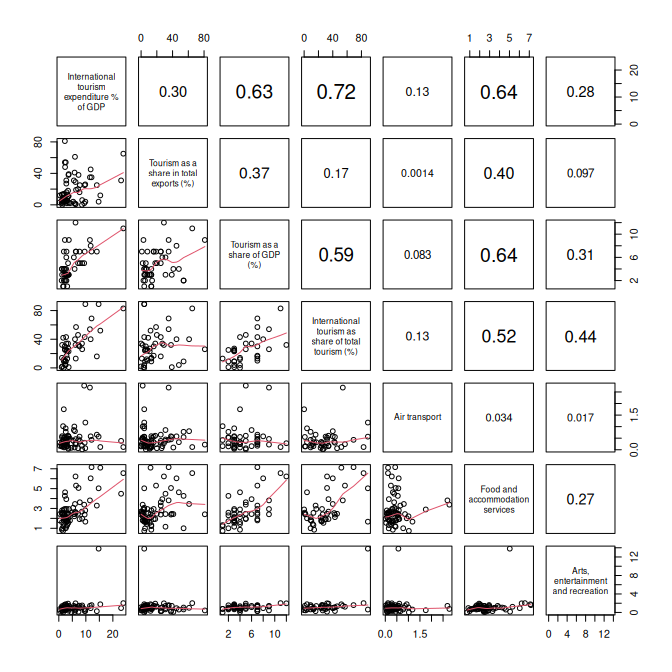
\includegraphics{p2_files/figure-latex/pairs-1} 

}

\caption{Correlations between tourism-related data. First: https://www.unwto.org/tourism-statistics/key-tourism-statistics. Second to fourth: https://www.unwto.org/tourism-data/international-tourism-and-covid-19. Fifth to seventh: OECD.}\label{fig:pairs}
\end{figure}

\newpage

\hypertarget{sector-shrinkage-as-a-result-of-the-pandemic}{%
\subsubsection{Sector shrinkage as a result of the pandemic}\label{sector-shrinkage-as-a-result-of-the-pandemic}}

For many countries, tourism was reduced not because of domestic mandates but because of reduced international travel. Therefore, the fraction of tourism that comes from abroad is a factor that can determine the impact of a pandemic on a country's GDP potentially independently of what happens within the country. (A useful model extension would be to include some dependence on country factors, e.g.~case numbers.)

We model mitigation via business closures, which are mandated per month and by sector. We represent openness with values \(x\) which range from 0 to 1, 1 representing maximum openness. To capture the impact of reduced international travel, we set the maximum openness of the food and accommodation services sector to be limited by international tourism as:

\[x_\tau = \min\{\hat{x}_\tau, 1+ y(z-1)\}\]

where \(\hat{x}_\tau\) is the openness of the sector in month \(\tau\) according to the schedule (i.e.~the mitigation strategy), \(y\) is the proportion of tourism that is international, and \(z\) is the fraction international tourism reduces to as a consequence of the pandemic. I.e. the tourism remaining is the domestic (\(1-y\)) plus that that comes in from abroad (\(yz\)).

Therefore, the contribution of the GVA of the food and accommodation services sector is limited either by the pandemic, or by the mitigation measures - whichever is lower.

\hypertarget{loss-of-international-tourists}{%
\subsubsection{Loss of international tourists}\label{loss-of-international-tourists}}

We model the distribution of \(z\) using data from 2020 (Figure \ref{fig:tourismhist}, bottom-right plot). We fit to it a log-normal distribution, and find mean value -1.39 and standard deviation 0.39 (Figure \ref{fig:ytd}). We use these values as inputs for all country models.

\begin{figure}

{\centering 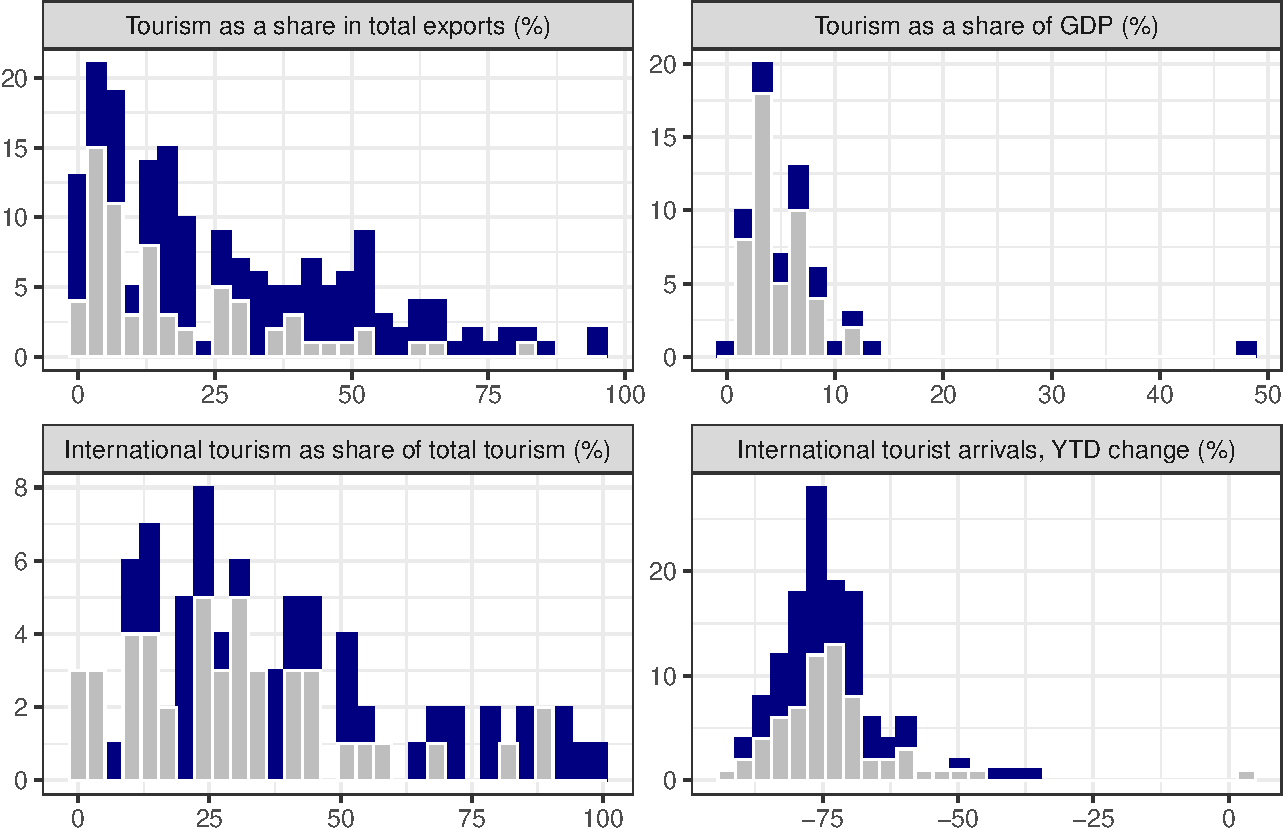
\includegraphics{p2_files/figure-latex/tourismhist-1} 

}

\caption{Distributions of tourism-related data from https://www.unwto.org/tourism-data/international-tourism-and-covid-19. In grey are the subset of countries for which we have GVA data by sector.}\label{fig:tourismhist}
\end{figure}

\begin{figure}

{\centering 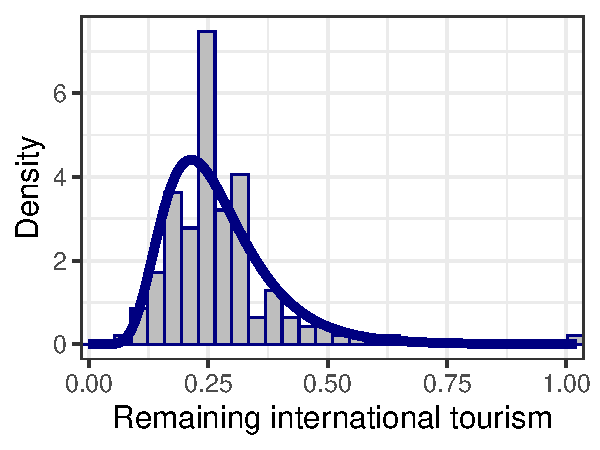
\includegraphics{p2_files/figure-latex/ytd-1} 

}

\caption{Fit of log-normal distribution to loss-of-tourism data.}\label{fig:ytd}
\end{figure}

\newpage

\hypertarget{dependence-on-international-tourism}{%
\subsubsection{Dependence on international tourism}\label{dependence-on-international-tourism}}

We model \(y\) as a function of the share of GDP that comes from the sector. Note that the data we have for this are biased towards high-income countries.

We write

\[y\sim\text{Beta}(\alpha(u),\beta(u))\]

where \(u\) is the fraction of GDP coming from the Food and accommodation sector. We learn three parameters \(p_1\), \(p_2\) and \(p_3\) to best fit the relationship between \(u\) and \(y\) in countries we have observations for:

\[p_1 = \alpha(u)+\beta(u)\]

\[p_2u + p_3 = \frac{\alpha(u)}{\alpha(u)+\beta(u)}\]

Here, \(p_1\) controls the variance of the distribution and \(p_2\) and \(p_3\) the linear relationship between \(u\) and \(y\). Using an optimisation routine in R we find \(p_1=5.93\), \(p_2=3.66\) and \(p_3=0.099\). Results are shown in Figure \ref{fig:sectortourism}. We use these values as inputs for all country models.

\begin{figure}
\centering
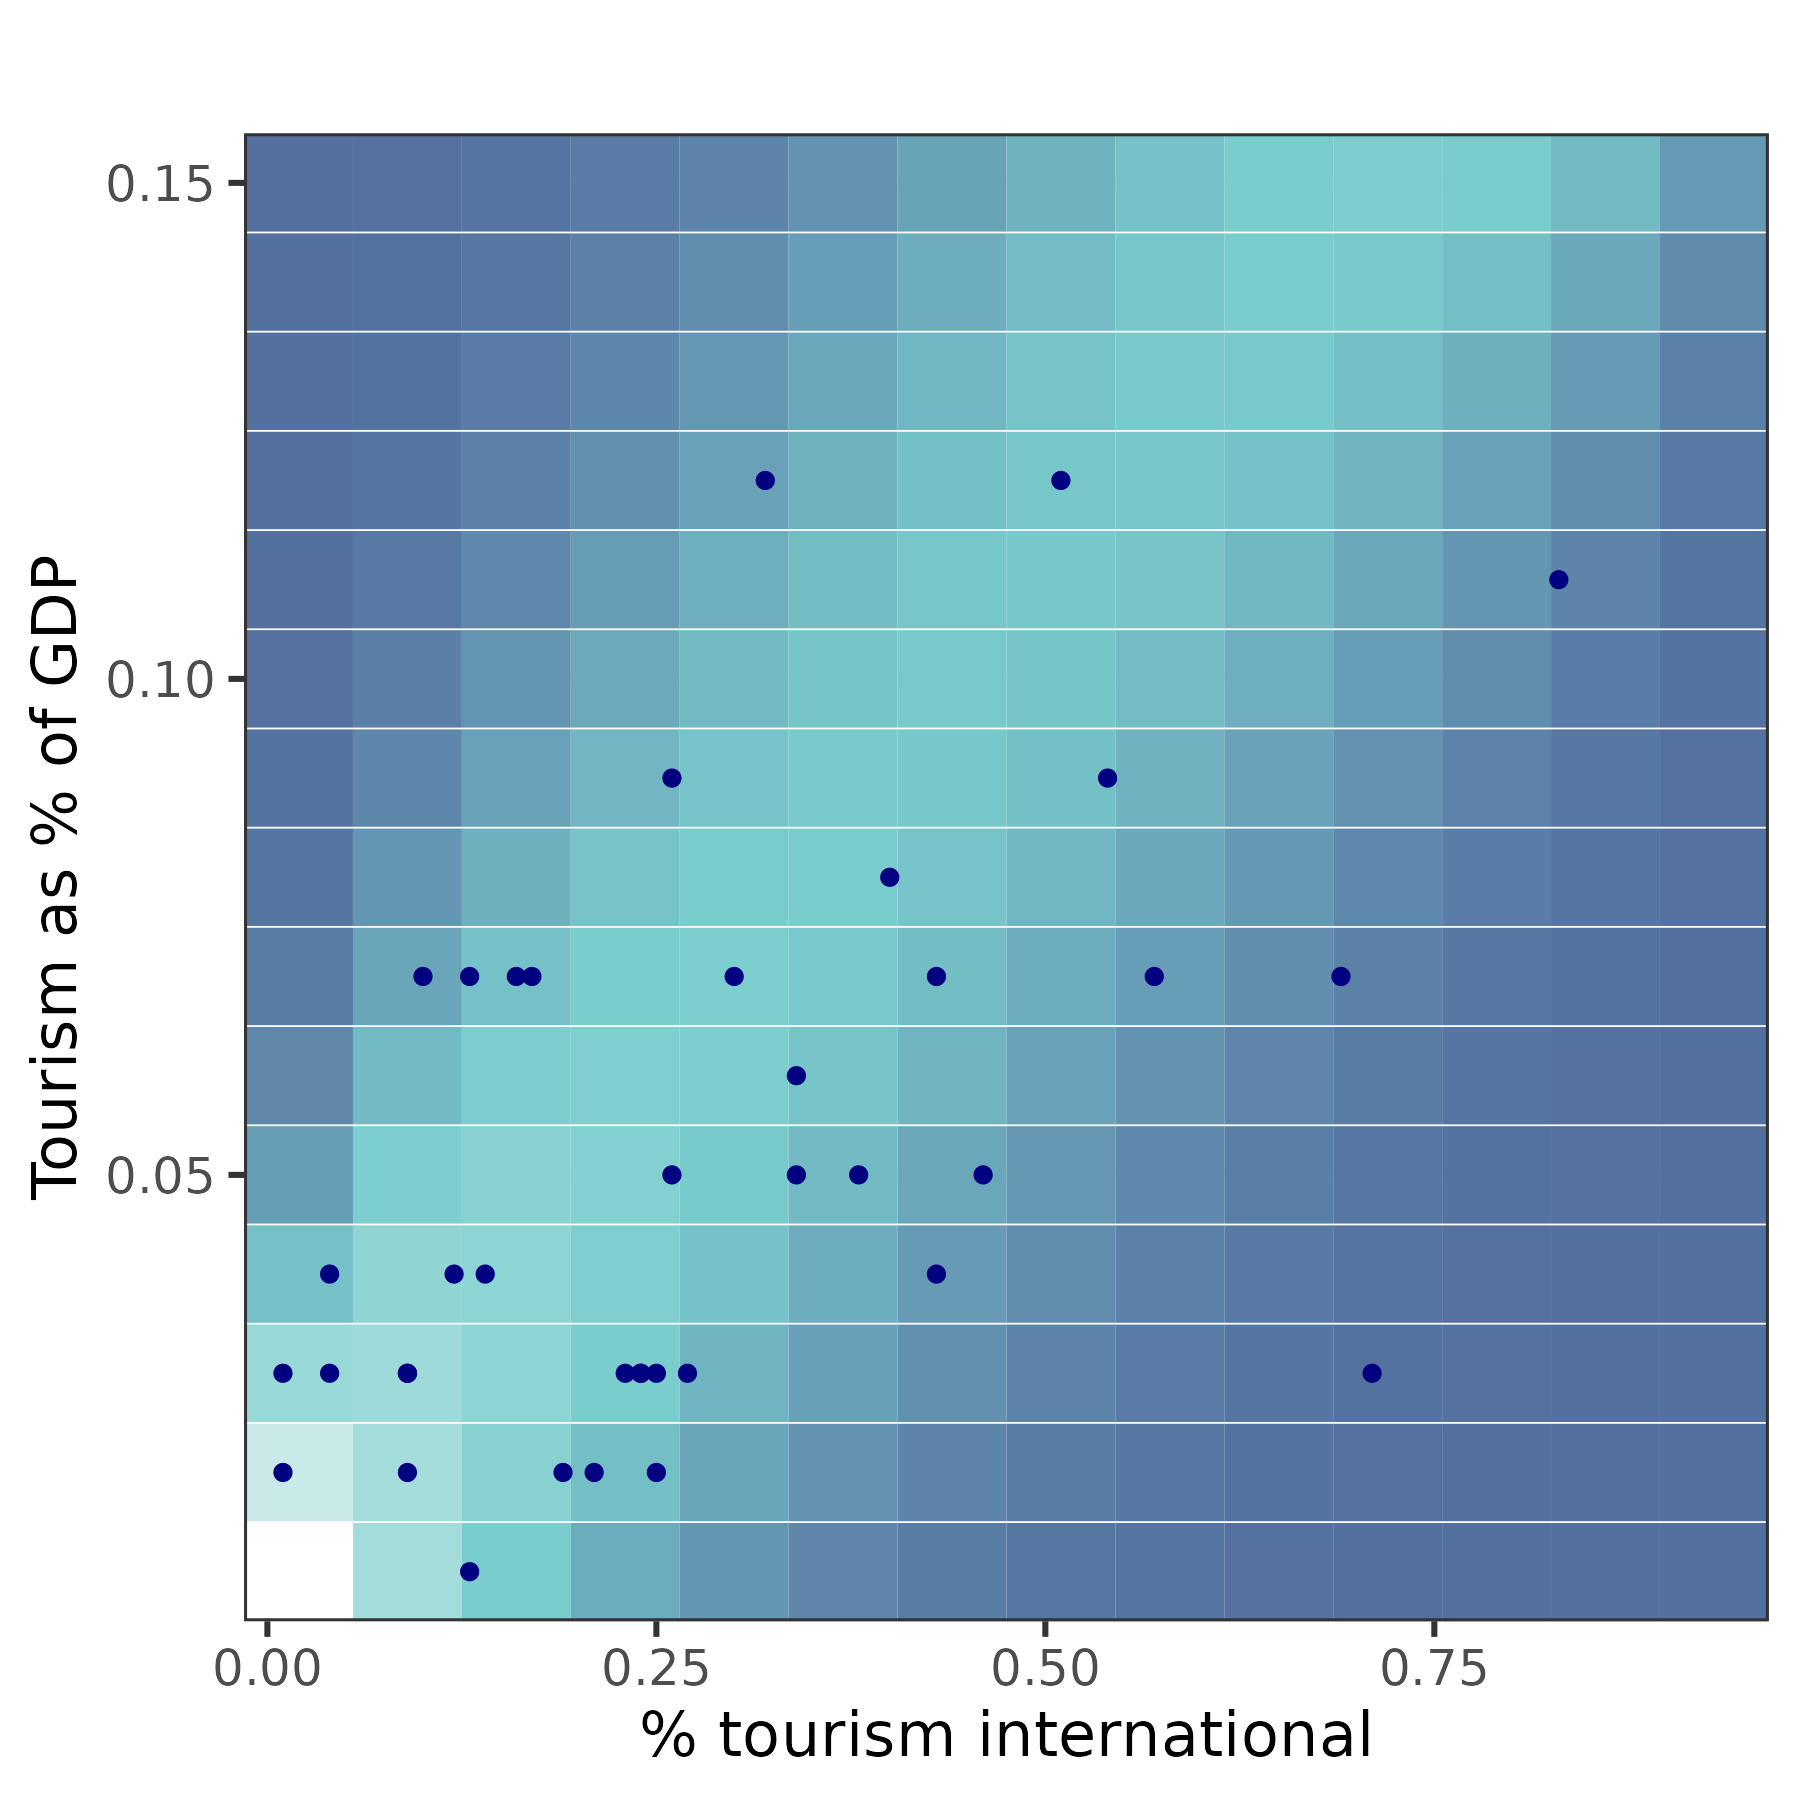
\includegraphics[width=0.6\textwidth,height=\textheight]{sectortourism.png}
\caption{\label{fig:sectortourism} Predicting the percentage of tourism that comes from abroad as a function of the size of the sector. Each row represents a beta distribution whose mean is determined by the size of the sector (u). Blue points show the data we have available (grey bars in Figure \ref{fig:tourismhist}).}
\end{figure}

\newpage

\hypertarget{sampling-sector-sizes}{%
\subsection{Sampling sector sizes}\label{sampling-sector-sizes}}

To learn about the impacts of changes to sector sizes, we use the following process to sample a baseline economic configuration.

\begin{enumerate}
\def\labelenumi{\arabic{enumi}.}
\tightlist
\item
  Sample a population distribution from all countries (within income group)
\item
  Sample new values for the population proportions of the Food and accommodation services and Agricultural workforces from uniform distributions bounded by the limits of the dataset
\item
  Scale the remaining sectors up or down proportionally to match the original total population size.
\end{enumerate}

\hypertarget{impact-of-sector-sizes}{%
\subsection{Impact of sector sizes}\label{impact-of-sector-sizes}}

The distribution of people among sectors of the workforce impacts the numbers of contacts made. In order to propagate these influences through the model, we sample a null distribution of contacts from the generating model and save the corresponding average number of candidate infectees (CI, where CI \(=R_0/\beta\)). Separately, we define a distribution over R\(_0\), e.g.~a normal distribution with its stated mean value and a coefficient of variation of 0.1. (E.g. for H1N1, with mean 1.58, the standard deviation given 95\% interval \{1.34, 2.04\} is 0.18 which is a coefficient of variation of 0.11 (Fraser et al. 2009).) Then, for each simulation, we compute the quantile of the CI distribution corresponding to the contacts generated, and select the corresponding quantile from the R\(_0\) distribution. Shown illustratively in Figure \ref{fig:candidateinfectees}.

\begin{figure}
\centering
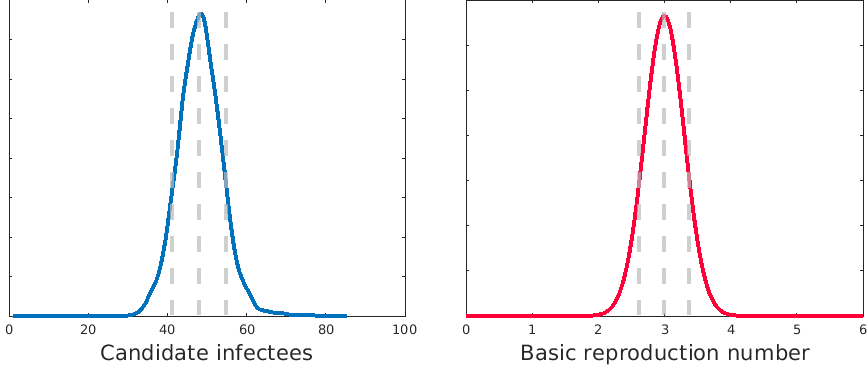
\includegraphics[width=0.8\textwidth,height=\textheight]{candidateinfectees.png}
\caption{\label{fig:candidateinfectees} The number of candidate infectees is mapped to the basic reproduction number \(R_0\) via matching quantiles from the simulated null distribution (left) to the parametric distribution (right). 10, 50 and 90\% quantiles shown.}
\end{figure}

\newpage

\hypertarget{internet-infrastructure}{%
\subsection{Internet infrastructure}\label{internet-infrastructure}}

For each sector in each country, we have the 90\% interval for the proportion of people who can work from home from (Gottlieb et al. 2021). We assume that the value we sample within the range is related to internet infrastructure, so that a low value in one sector implies low values in all sectors. We:

\begin{itemize}
\tightlist
\item
  Take the subset of countries in the income group (LLMIC / MIC / HIC)
\item
  Take the minimum of the lower bounds by sector (5\%)
\item
  Take the maximum of the upper bounds by sector (95\%)
\item
  Sample from a uniform distribution between these bounds, taking the same quantile for each sector
\item
  Use the same quantile again for internet coverage in computing the effectiveness of remote learning
\end{itemize}

\hypertarget{remote-teaching}{%
\subsubsection{Remote teaching}\label{remote-teaching}}

For the value of a year of education, we use the method of (Psacharopoulos, Collis, and Patrinos 2021). The loss due to school closure is

\[L = \text{PV}\cdot Y\cdot \alpha\cdot r\cdot S\cdot \beta\]

where PV is the present value of lost earnings:

\[\text{PV} =  \frac{1-(1+d)^{-n}}{d}\]

for discount rate \(d=0.03\) and expected number of years of work \(n=45\). \(Y\) is mean annual earnings, \(\alpha\) is the fraction of the year schools are closed: \[\alpha=\frac{1}{12}\sum_{\tau=1}^{12}1-x_{ed,\tau},\] \(r=0.08\) is the rate of return for one year, \(S\) is the total number of students, and \(\beta\) is the proportion of students affected. We take \(\beta=1-0.86I\) to be the complement fraction of internet coverage \(I\) (Figure \ref{fig:internet}) multiplied by 0.86, to match values for the Philippines: it has 43\% internet coverage and effectiveness of remote education was estimated to be 37\% (National Economic and Development Authority 2021).

\begin{figure}
\centering
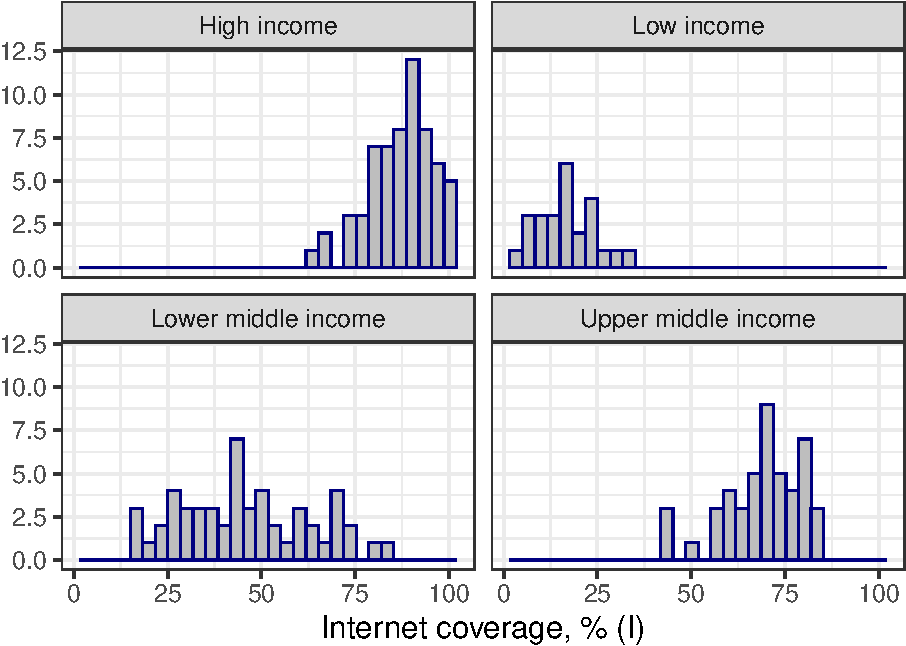
\includegraphics{p2_files/figure-latex/internet-1.pdf}
\caption{\label{fig:internet}Internet access by income level. World Bank data for 2019.}
\end{figure}

We model the Figure \ref{fig:internet} values with Beta distributions. For LLMICs, we have parameters 1.78 and 3.11. For MICs, we have parameters 3.77 and 2.91. For HICs, we have parameters 9.57 and 1.39.

We estimate the average annual income per working-age adult as the total GVA multiplied by the fraction of GVA that goes to labour divided by the number of working-age adults. For the fraction of GVA that goes to labour we use PWT estimates from 2011 (Figure \ref{fig:labsh}). (This correction might lead us to underestimate the impact of education: perhaps GNI per working-age adult is better than average income among working-age adults. E.g. suppose Country A and Country B have the same GVA and the same number of workers, where GVA = labour compensation + capital. And suppose Country A splits its GVA between labour and capital with ratio 1:2, and Country B with ratio 2:1. Then the value of education in Country B is twice that in Country A, because we are only counting the income contribution to the economy. If we wanted to estimate the impact on the economy, we should use the whole GVA, not just the labour share.)

\begin{figure}
\centering
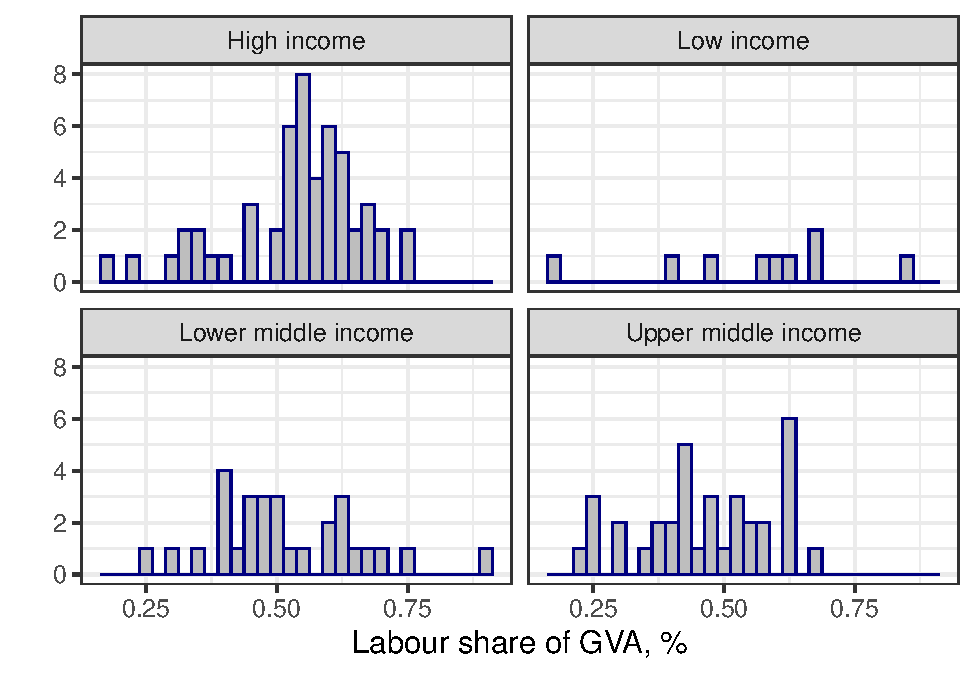
\includegraphics{p2_files/figure-latex/labsh-1.pdf}
\caption{\label{fig:labsh}Fraction of GVA that goes to labour (PWT, 2011).}
\end{figure}

We model these values with Beta distributions. For LLMICs, we have parameters 5.09 and 4.51. For MICs, we have parameters 6.29 and 6.54. For HICs, we have parameters 7.97 and 6.87.

\newpage

\hypertarget{hospital-capacity}{%
\subsection{Hospital capacity}\label{hospital-capacity}}

\begin{figure}
\centering
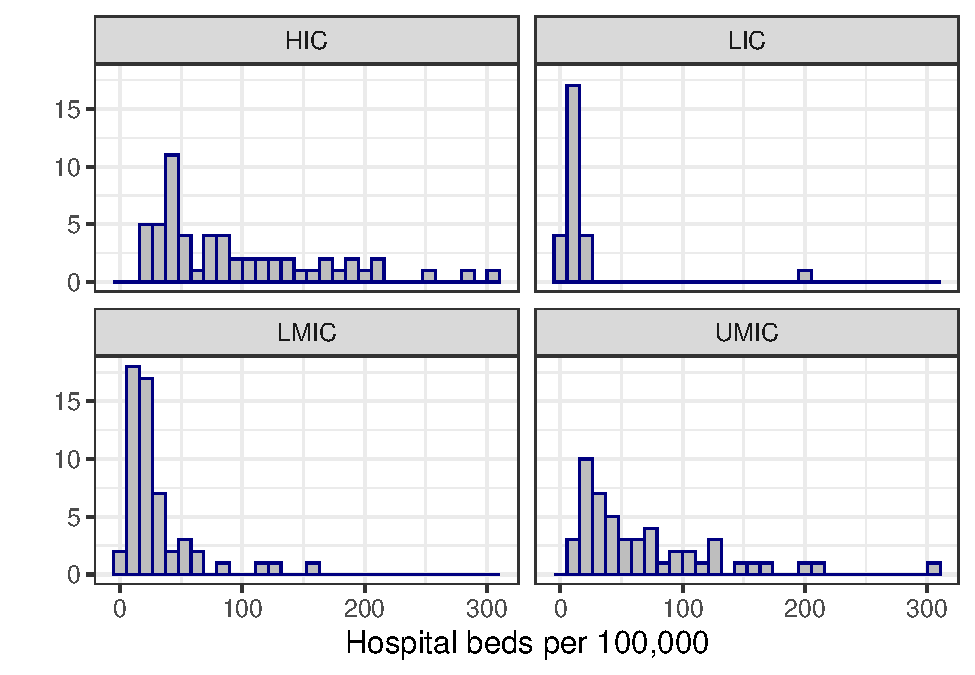
\includegraphics{p2_files/figure-latex/hmax-1.pdf}
\caption{\label{fig:hmax}Fraction of GVA that goes to labour (PWT, 2011).}
\end{figure}

We model these values with gamma distributions. For LLMICs, we have parameters 1.3 and 0.05. For MICs, we have parameters 1.36 and 0.03. For HICs, we have parameters 2.05 and 0.02.

\hypertarget{comparison-of-model-results-for-sars-cov-2-pre-alpha-to-2020-data}{%
\section{Comparison of model results for SARS-CoV-2 (pre-alpha) to 2020 data}\label{comparison-of-model-results-for-sars-cov-2-pre-alpha-to-2020-data}}

Our model has not been calibrated to fit any observed economic outcomes in general or for any specific country. However, the distributions for the pre-alpha profile of SARS-CoV-2 should align to some extent with data pertaining to 2020, as many of the inputs to the model were taken from this period.

\hypertarget{gdp-loss}{%
\subsection{GDP loss}\label{gdp-loss}}

\begin{figure}
\centering
\includegraphics{p2_files/figure-latex/gdpdata-1.pdf}
\caption{\label{fig:gdpdata}GDP loss: loss in 2020 as a percentage of 2019 GDP (IMF). NB: data are annual, so the loss is for the year starting January 2020. We would prefer to present data for April 2020 to March 2021 but these data are unavailable for most countries. The outlier is Guyana.}
\end{figure}

\begin{figure}
\centering
\includegraphics{p2_files/figure-latex/gdpdatallmic-1.pdf}
\caption{\label{fig:gdpdatallmic}GDP loss: loss in 2020 as a percentage of 2019 GDP (IMF) for low- and lower-middle-income countries with densities from the model shown by strategy. NB: data are annual, so the loss is for the year starting January 2020. We would prefer to present data for April 2020 to March 2021 but these data are unavailable for most countries.}
\end{figure}

\begin{figure}
\centering
\includegraphics{p2_files/figure-latex/gdpdatamic-1.pdf}
\caption{\label{fig:gdpdatamic}GDP loss: loss in 2020 as a percentage of 2019 GDP (IMF) for upper- and lower-middle-income countries with densities from the model shown by strategy. NB: data are annual, so the loss is for the year starting January 2020. We would prefer to present data for April 2020 to March 2021 but these data are unavailable for most countries. The outlier is Guyana.}
\end{figure}

\begin{figure}
\centering
\includegraphics{p2_files/figure-latex/gdpdatahic-1.pdf}
\caption{\label{fig:gdpdatahic}GDP loss: loss in 2020 as a percentage of 2019 GDP (IMF) for high-income countries with densities from the model shown by strategy. NB: data are annual, so the loss is for the year starting January 2020. We would prefer to present data for April 2020 to March 2021 but these data are unavailable for most countries.}
\end{figure}

\newpage

\hypertarget{school-closure}{%
\subsection{School closure}\label{school-closure}}

\begin{figure}
\centering
\includegraphics{p2_files/figure-latex/schooldata-1.pdf}
\caption{\label{fig:schooldata}Extent of school closure. Horizontal lines (one per country) show the duration of the first year spent with schools partially closed. The space to the left of the line represents the duration schools were open. The space to the right of the line represents the duration schools were closed. (UNESCO)}
\end{figure}

\newpage

\hypertarget{value-of-lives-lost}{%
\subsection{Value of lives lost}\label{value-of-lives-lost}}

\begin{figure}
\centering
\includegraphics{p2_files/figure-latex/lives-1.pdf}
\caption{\label{fig:lives}Valued loss of life, using IHME estimates (``cumulative deaths'') for the first year of accumulated deaths. The value of a statistical life used is 160 times GDP per capita. (This means that a 0.625\% mortality rate is worth 100\% of GDP.)}
\end{figure}

\end{document}
